\section{Treinamento de modelos}

\begin{frame}	
	\begin{block}{Treinamento}	
		\begin{itemize}
			\item O processo de treinamento é único para cada modelo mas a forma como se treina um modelo é parecida
			\item Os dados são dividos em treino (70\%) e teste (30\%)
			\item O conjunto de treino é apresentado ao modelo com os rótulos de cada observação
			\item Tipicamente usa-se uma validação cruzada para treinar o modelo
		\end{itemize}		
	\end{block}
\end{frame}

\begin{frame}	
	\begin{block}{Validação}	
		\begin{itemize}
			\item O modelo é validado com o conjunto de teste, o qual não deve exibir os rótulos para o modelo
			\item Alguma métrica de validação de modelos é usada, por exemplo, precisão $\dfrac{VP}{VP + FP}$
		\end{itemize}
				\begin{figure}[!htb]
			\centering	  				
			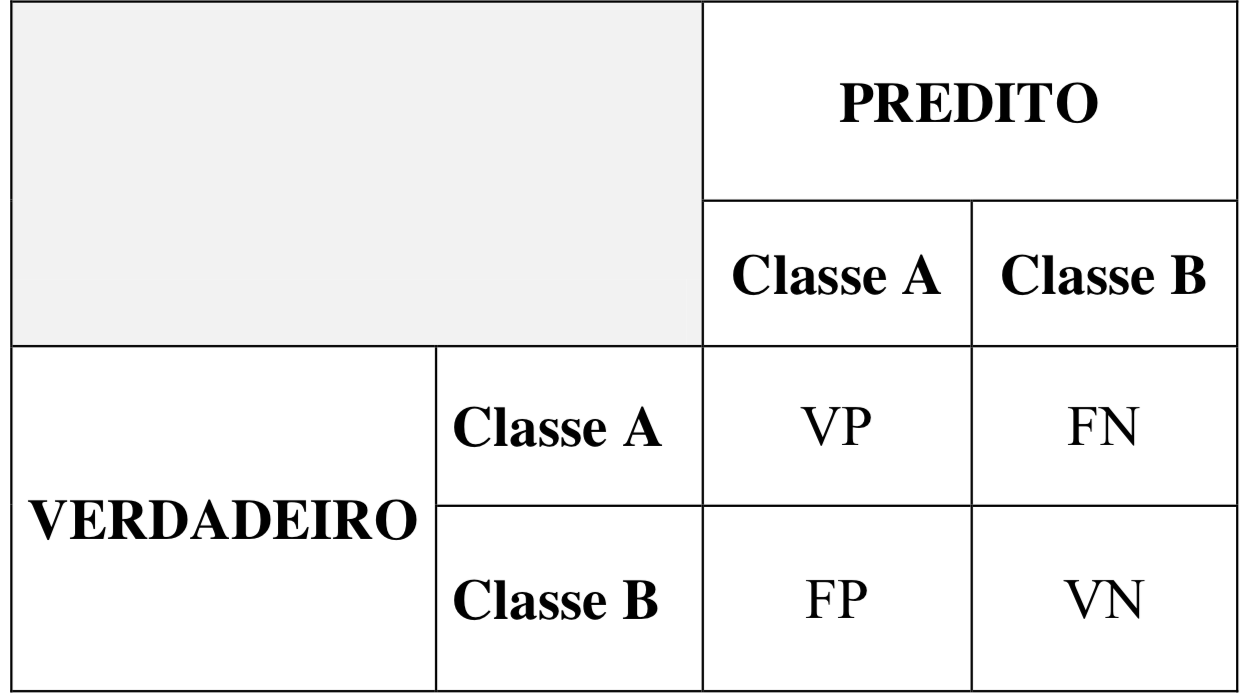
\includegraphics[height=4cm, width = 10cm]{./pic/matrizConfusao.png}
			\caption{Obtido no link: \href{http://www.scielo.br/pdf/eagri/v33n6/19.pdf}{Scielo} }
			\label{fig_matriz_confusao}
		\end{figure}	
	\end{block}
\end{frame}